\subsection{Временные ряды}

        На временных рядах можно продемонстрировать как различные виды шума влияют на поведение системы.

        На рисунке \ref{time_series_x_0_06_a_1_b_0_56} изображено поведение модели без добавления каких-либо шумов. Видно, что значения переменной \(x\) с течением времени стабилизируются. Численность популяции фактически остается неизменной.

        \begin{figure}
            \centering
            \subfloat[Для модели (\ref{origin})]{
                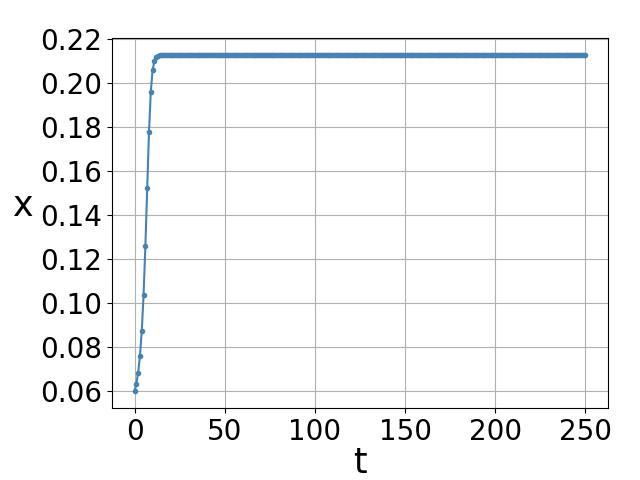
\includegraphics[width=0.5\textwidth]{stochastic/images/time_series_x_0_06_a_1_b_0_56.jpg}
                \label{time_series_x_0_06_a_1_b_0_56}
            }
            \subfloat[Для модели (\ref{alpha_chaos})]{
                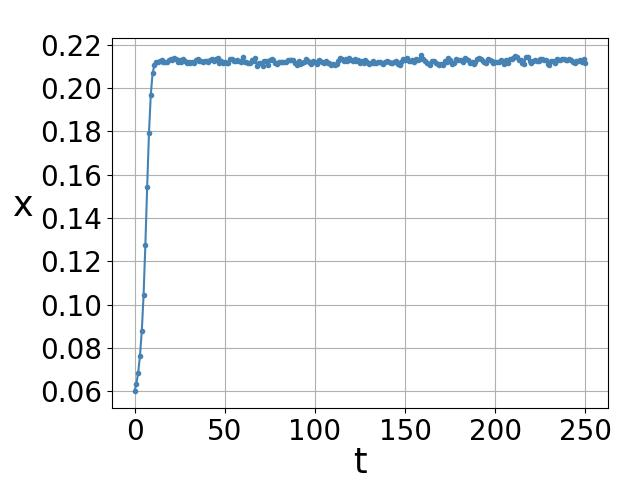
\includegraphics[width=0.5\textwidth]{stochastic/images/time_series_x_0_06_a_1_b_0_56_alpha_chaos_epsilon_0_004.jpg}
                \label{time_series_x_0_06_a_1_b_0_56_alpha_chaos_epsilon_0_004}
            }  

            \subfloat[Для модели (\ref{beta_chaos})]{
                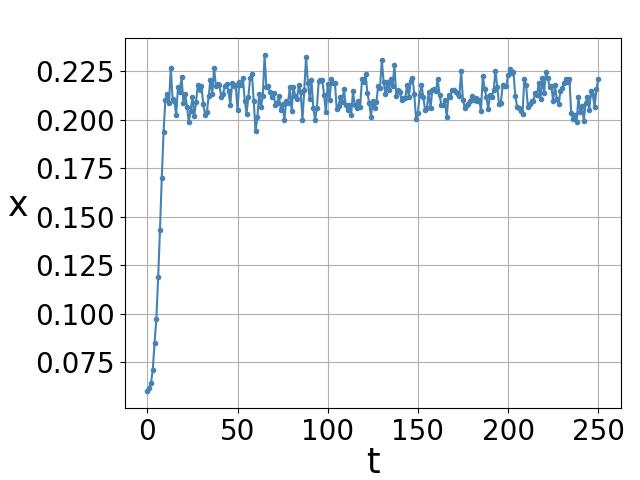
\includegraphics[width=0.5\textwidth]{stochastic/images/time_series_x_0_06_a_1_b_0_56_beta_chaos_epsilon_0_004.jpg}
                \label{time_series_x_0_06_a_1_b_0_56_beta_chaos_epsilon_0_004}
            }
            \subfloat[Для модели (\ref{additive_chaos})]{
                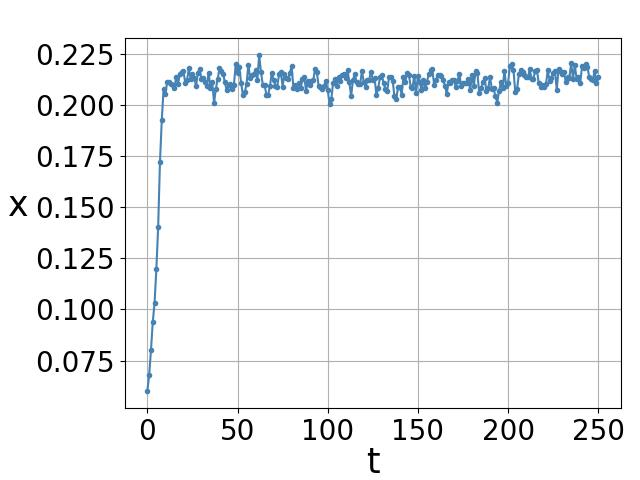
\includegraphics[width=0.5\textwidth]{stochastic/images/time_series_x_0_06_a_1_b_0_56_additive_chaos_epsilon_0_004.jpg}
                \label{time_series_x_0_06_a_1_b_0_56_additive_chaos_epsilon_0_004}
            }
            
            \caption{Временные ряды при \(\alpha = 1, \beta = 0.56, x_0 = 0.06, \varepsilon = 0.004\)}
        \end{figure}

        Далее на рисунках \ref{time_series_x_0_06_a_1_b_0_56_alpha_chaos_epsilon_0_004}, \ref{time_series_x_0_06_a_1_b_0_56_beta_chaos_epsilon_0_004}, \ref{time_series_x_0_06_a_1_b_0_56_additive_chaos_epsilon_0_004} представлены временные ряды для различных видов шума: 

        \begin{enumerate}[a)]
            \setcounter{enumi}{1}
            \item \(\alpha\)-шум
            \item \(\beta\)-шум
            \item аддитивный шум
        \end{enumerate}

        Все варианты рассматриваются с одной и той же интенсивностью шума \(\varepsilon = 0.004\). 
        
        Мы видим, что вид шума влияет на величину разброса значений численности популяции. \comment{Приплети сюда дисперсию.} И если раньше численность популяции стабилизировалась и переставала хоть сколько-нибудь меняться, то сейчас численность постоянно всегда колеблется, но как можно заметить, она меняется в рамках некоторого коридора значений. Численность популяции в общем то не растет и не уменьшается на какую-то значительную величину. Но такое поведение наблюдается не всегда.

        \comment{малый шум будет оказывать незначительное влияние, а большой - огромное.}

        \comment{Можно взять оригинальный временной ряд и на него сверху наложить временной ряд с шумом.}

        \comment{Хорошая фраза: индуцированный шумом переход}

        Для того чтоб продемонстрировать другое возможное поведение, давайте увеличим интенсивность шума. Пускай теперь \(\varepsilon = 0.04\). Рассмотрим рисунок \ref{time_series_x_0_06_a_1_b_0_56_beta_chaos_epsilon_0_04_fall}. Здесь мы видим ситуацию, когда шум оказал негативное влияние на численность популяции. Но опять же все не так просто. Если мы еще раз запустим алгоритм, который просчитывает нашу модель, то мы увидим, что популяция успешно выживала на протяжении анализируемого интервала времени. Данный пример проиллюстрирован на картинке \ref{time_series_x_0_06_a_1_b_0_56_beta_chaos_epsilon_0_04_alive}. Аналогичные эффекты можно наблюдать и при других видах шума.

        \comment{Примерно в \(t = 50\) обе популяции были близки к вымиранию, но одна выжила, а вторая нет. "Одно рисовое зернышко может склонить чашу весов" (с) какой-то мультик.}

        \begin{figure}
            \centering
            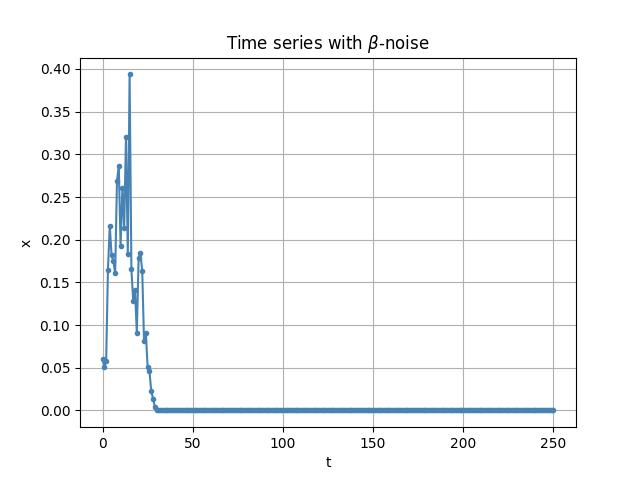
\includegraphics[width=\textwidth]{stochastic/images/time_series_x_0_06_a_1_b_0_56_beta_chaos_epsilon_0_04_fall.jpg}
        
            \captionsetup{justification=centering}
            \caption{Временной ряд модели (\ref{beta_chaos}) при \(\beta = 0.56, \alpha = 1, x_0 = 0.06, \varepsilon = 0.04\)}
            \label{time_series_x_0_06_a_1_b_0_56_beta_chaos_epsilon_0_04_fall}
        \end{figure}

        \begin{figure}
            \centering
            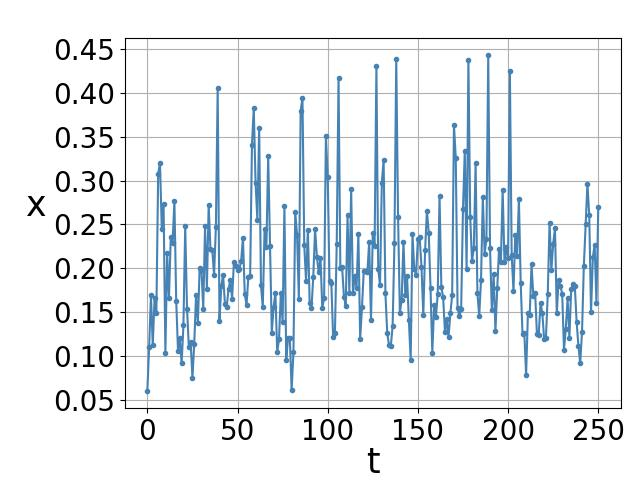
\includegraphics[width=\textwidth]{stochastic/images/time_series_x_0_06_a_1_b_0_56_beta_chaos_epsilon_0_04_alive.jpg}
        
            \captionsetup{justification=centering}
            \caption{Временной ряд модели (\ref{beta_chaos}) при \(\beta = 0.56, \alpha = 1, x_0 = 0.06, \varepsilon = 0.04\)}
            \label{time_series_x_0_06_a_1_b_0_56_beta_chaos_epsilon_0_04_alive}
        \end{figure}

        Анализируя вышесказанное можно сказать, что при добавлении в модель случайных событий ее поведение становится непредсказуемым. Одно незначительное изменение может кардинально повлиять на ход развития событий. 

        \comment{рассматривать как в том семестре все возможные варианты поведения системы в зависимости от начальной точки думаю не надо и так все понятно.}